\documentclass[11pt,a4paper]{article}

% ── Packages ──
\usepackage[utf8]{inputenc}
\usepackage[T1]{fontenc}
\usepackage{amsmath,amssymb,amsthm}
\usepackage{mathtools}
\usepackage{graphicx}
\usepackage[margin=1in]{geometry}
\usepackage{booktabs}
\usepackage{array}
\usepackage{hyperref}
\usepackage{xcolor}
\usepackage{enumitem}

% ── Theorem environments ──
\newtheorem{theorem}{Theorem}[section]
\newtheorem{corollary}[theorem]{Corollary}
\newtheorem{definition}[theorem]{Definition}
\newtheorem{remark}[theorem]{Remark}

% ── Hyperlinks ──
\hypersetup{colorlinks=true, linkcolor=blue!70!black, citecolor=blue!70!black, urlcolor=blue!60!black}

% ── Shorthand ──
\newcommand{\Qk}{Q_k}
\newcommand{\Fp}{\mathbb{F}_p}
\newcommand{\Fpstar}{\mathbb{F}_p^*}
\newcommand{\ZZ}{\mathbb{Z}}
\newcommand{\QQ}{\mathbb{Q}}

\begin{document}

% ═══════════════════════════ TITLE ═══════════════════════════
\begin{center}
\vspace*{1cm}
{\LARGE\bfseries Prime Constellations of $n^k - (n-1)^k$:}\\[6pt]
{\Large\bfseries Algebraic Obstructions, Bateman--Horn Verification,}\\[4pt]
{\Large\bfseries and the Non-Monotonicity of Maximum Constellation Lengths}\\[20pt]
{\large\bfseries Ruqing Chen}\\[6pt]
GUT Geoservice Inc., Montreal, Canada\\[3pt]
\href{mailto:ruqing@hotmail.com}{\textcolor{blue!70!black}{ruqing@hotmail.com}}\\[10pt]
{\textcolor{gray}{February 2026}}
\end{center}

\vspace{20pt}

% ═══════════════════════════ ABSTRACT ═══════════════════════════
\section*{Abstract}

\noindent\textbf{Abstract.}
We investigate the polynomial family $\Qk(n) = n^k - (n-1)^k$ for prime exponents $k = 3, 5, 7, 11, 13$, enumerating all prime values for $n \le 10^8$ and searching for consecutive prime constellations up to $n \le 2\times 10^9$. We prove that the true maximum constellation length is bounded above by $L(k)$, defined as the longest run of non-forbidden residues modulo the smallest splitting prime $p_0 \equiv 1 \pmod{k}$, yielding $L(3) = 3$, $L(5) = 6$, $L(7) = 17$, $L(11) = 4$, $L(13) = 8$. All five upper bounds are confirmed computationally: no constellation exceeding $L(k)$ occurs. The Bateman--Horn conjecture is verified to $0.2\%$ accuracy across four polynomial degrees $(4, 6, 10, 12)$. We discover that $L(k)$ is non-monotonic in~$k$, controlled by the forbidden density $\rho(k) = (k-1)/p_0(k)$, and identify striking residue-locking phenomena where all quadruplets are confined to as few as 2 admissible classes modulo~$p_0$.

\medskip
\noindent\textbf{Keywords:} prime-producing polynomials, Bateman--Horn conjecture, prime constellations, cyclotomic splitting, algebraic obstructions

\medskip
\noindent\textbf{2020 Mathematics Subject Classification:} 11N32, 11N05, 11C08, 11Y35

% ═══════════════════════════ 1. INTRODUCTION ═══════════════════════════
\section{Introduction}

For a prime number~$k$, the polynomial $\Qk(n) = n^k - (n-1)^k$ is a monic polynomial of degree $k-1$ in~$n$. It arises naturally as the first difference of consecutive perfect $k$-th powers. When expanded via the binomial theorem,
\[
  \Qk(n) = \sum_{j=0}^{k-1} \binom{k}{j} (-1)^{k-1-j}\, n^j,
\]
where $\binom{k}{j}$ denotes the binomial coefficient. For instance, $Q_3(n) = 3n^2 - 3n + 1$ is a quadratic whose prime values are known as \emph{Cuban primes} (OEIS~A002407; see~\cite{ribenboim, cunningham}), $Q_5(n) = 5n^4 - 10n^3 + 10n^2 - 5n + 1$ is a quartic, and $Q_7(n) = 7n^6 - 21n^5 + 35n^4 - 35n^3 + 21n^2 - 7n + 1$ is of degree~6. When $k$ is prime, $\Qk(n)$ coincides with the homogeneous cyclotomic polynomial $\Phi_k(n,\, n-1) = (n^k - (n-1)^k)/(n - (n-1))$ evaluated at the pair $(n,\, n-1)$, connecting our investigation to the arithmetic of cyclotomic fields.

A natural question, with deep connections to the distribution of primes represented by polynomials, is: for how many consecutive values of $n$ can $\Qk(n)$ be simultaneously prime? We call $m$ consecutive integers $n, n+1, \ldots, n+m-1$ such that $\Qk(n), \Qk(n+1), \ldots, \Qk(n+m-1)$ are all prime an \emph{$m$-tuplet} or \emph{$m$-constellation}. We define $L(k)$ to be the supremum of such~$m$. Note that our constellations are consecutive in the \emph{parameter}~$n$, not in the natural number line: for instance, $Q_3(2) = 7$ and $Q_3(3) = 19$ form a 2-tuplet even though 7 and~19 are separated by other primes.

The Bateman--Horn conjecture~\cite{batemanhorn}, a quantitative refinement of Schinzel's Hypothesis~H~\cite{schinzel}, provides a prediction for the number of integers $n \le N$ for which a given set of polynomials simultaneously takes prime values. For a single irreducible polynomial~$f$ of degree~$d$, it predicts
\[
  \pi_f(N) \;\sim\; C \cdot \sum_{n=2}^{N} \frac{1}{\ln|f(n)|},
\]
where $C = \prod_{p\;\mathrm{prime}} \frac{1 - \omega(p)/p}{1 - 1/p}$ and $\omega(p)$ denotes the number of roots of~$f$ modulo~$p$. This constant captures the local obstructions: when $\omega(p) = 0$ for many small primes, $C$ exceeds~1 and the polynomial produces primes more frequently than a ``generic'' polynomial of the same degree.

In this paper, we establish three main results.
\emph{First}, we prove that $\Qk(n) \equiv 0 \pmod{p}$ if and only if $p \equiv 1 \pmod{k}$, with exactly $k-1$ roots (Theorem~\ref{thm:sieving}). This immediately implies $C(k) > 1$ for all prime~$k$.
\emph{Second}, we derive a rigorous upper bound $L(k)$ for the constellation length in terms of the forbidden residue pattern modulo the smallest splitting prime $p_0(k)$ (Theorem~\ref{thm:admissibility}), and prove that $L(k)$ is non-monotonic (Theorem~\ref{thm:nonmono}). Subject to the Bateman--Horn conjecture, $L(k)$ is also a lower bound, i.e., constellations of length exactly $L(k)$ exist.
\emph{Third}, we provide large-scale computational verification for $k = 3, 5, 7, 11, 13$, encompassing over 15~million primes and 19,000 constellations. In each case, constellations of length $L(k)$ are found, and none of length $L(k)+1$ occur.

% ═══════════════════════════ 2. ALGEBRAIC FRAMEWORK ═══════════════════════════
\section{Algebraic Framework}

\subsection{Splitting behavior of $\Qk(n)$ modulo primes}

\begin{theorem}[Algebraic Sieving Law]\label{thm:sieving}
Let $k$ be an odd prime and $p$ a prime with $p \ne k$. Then $\Qk(n) \equiv 0 \pmod{p}$ has solutions if and only if $p \equiv 1 \pmod{k}$. When solutions exist, there are exactly $k-1$ distinct roots modulo~$p$.
\end{theorem}

\begin{proof}
We work in $\Fp = \ZZ/p\ZZ$. Consider $\Qk(n) = n^k - (n-1)^k$. If $p \mid (n-1)$, then $\Qk(n) \equiv n^k \equiv 1^k = 1$, which is nonzero. So we may assume $\gcd(n-1, p) = 1$ and set $m = n \cdot (n-1)^{-1}$ in~$\Fpstar$. Then
\[
  \Qk(n) = (n-1)^k \cdot (m^k - 1).
\]
Since $(n-1)^k \ne 0$, the vanishing of $\Qk(n)$ is equivalent to $m^k = 1$ in~$\Fpstar$. The multiplicative group $\Fpstar$ is cyclic of order $p-1$, so the equation $x^k = 1$ has exactly $\gcd(k,\, p-1)$ solutions. Since $k$ is prime, this is $k$ if $k \mid (p-1)$, and~$1$ otherwise.

When $k \nmid (p-1)$, i.e., $p \not\equiv 1 \pmod{k}$, the only solution to $m^k = 1$ is $m = 1$. But $m = 1$ means $n \equiv n - 1$, i.e., $0 \equiv -1 \pmod{p}$, giving $p = 1$, a contradiction. Hence $\Qk(n)$ has no roots.

When $k \mid (p-1)$, i.e., $p \equiv 1 \pmod{k}$, there are $k$ solutions to $m^k = 1$. Among these, $m = 1$ yields no valid~$n$ (as shown above). The remaining $k-1$ nontrivial $k$-th roots of unity each determine a unique $n$ via $n \equiv m(m-1)^{-1} \pmod{p}$, where the invertibility of $m-1$ is guaranteed since $m \ne 1$. This produces exactly $k-1$ distinct roots.
\end{proof}

\begin{remark}\label{rem:pk}
For the case $p = k$, Fermat's little theorem gives $n^k \equiv n \pmod{k}$ and $(n-1)^k \equiv n-1 \pmod{k}$, hence $\Qk(n) = n^k - (n-1)^k \equiv n - (n-1) \equiv 1 \pmod{k}$. Thus $k$ never divides $\Qk(n)$. Combined with Theorem~\ref{thm:sieving}, this shows that \emph{every} prime factor of $\Qk(n)$ must be congruent to~$1$ modulo~$k$.
\end{remark}

\begin{remark}\label{rem:irred}
The polynomial $\Qk(n)$ is irreducible over~$\ZZ$ for every prime~$k$. To see this, note that the substitution $n = x/(x-1)$ transforms $\Qk(n)$ (up to a unit in $\ZZ[x,x^{-1}]$) into the $k$-th cyclotomic polynomial $\Phi_k(x) = x^{k-1} + x^{k-2} + \cdots + 1$, which is irreducible over~$\QQ$ by the classical theorem of Gauss (see~\cite{washington}, Theorem~2.5). Irreducibility is a prerequisite for the Bateman--Horn conjecture to predict infinitely many prime values.
\end{remark}

\begin{corollary}\label{cor:Cbig}
For each prime~$k$, all primes $p < p_0(k) = \min\{q \text{ prime} : q \equiv 1 \pmod{k}\}$ contribute no sieving to $\Qk(n)$. Consequently, the Bateman--Horn constant satisfies $C(k) > 1$ for all prime $k \ge 3$.
\end{corollary}

\begin{proof}
In the Euler product for $C(k)$, the factor for prime~$p$ is $(1 - \omega(p)/p)/(1 - 1/p)$. When $\omega(p) = 0$ (which holds for all $p \not\equiv 1 \pmod{k}$ and $p \ne k$), this factor equals $1/(1 - 1/p) > 1$. Since there are infinitely many such primes, their product diverges, and the convergence of the full product to a value $C(k) > 1$ follows from the compensation by primes $p \equiv 1 \pmod{k}$ where $\omega(p) = k - 1$.
\end{proof}

We verified Theorem~\ref{thm:sieving} computationally for all primes $p < 5000$ and all $k \in \{3, 5, 7, 11, 13\}$, finding zero exceptions. The following table records the forbidden residues for each~$k$:

\begin{table}[ht]
\centering
\caption{Forbidden residues for each prime exponent~$k$.}\label{tab:forbidden}
\smallskip
\begin{tabular}{cccc}
\toprule
$k$ & $p_0(k)$ & Forbidden residues $F(k) \bmod p_0$ & $|F(k)|$ \\
\midrule
3  & 7  & $\{2, 6\}$ & 2 \\
5  & 11 & $\{4, 5, 7, 8\}$ & 4 \\
7  & 29 & $\{3, 5, 6, 24, 25, 27\}$ & 6 \\
11 & 23 & $\{2, 3, 4, 9, 11, 13, 15, 20, 21, 22\}$ & 10 \\
13 & 53 & $\{3, 7, 16, 20, 22, 23, 31, 32, 34, 38, 47, 51\}$ & 12 \\
\bottomrule
\end{tabular}
\end{table}

\subsection{Maximum constellation length}

\begin{definition}\label{def:density}
For prime~$k$, let $p_0(k) = \min\{p \text{ prime} : p \equiv 1 \pmod{k}\}$ and $F(k) = \{n \bmod p_0 : \Qk(n) \equiv 0 \pmod{p_0}\}$. The \emph{forbidden density} is $\rho(k) = |F(k)|/p_0(k) = (k-1)/p_0(k)$.
\end{definition}

\begin{theorem}[Admissibility Bound]\label{thm:admissibility}
Let $L(k)$ be the length of the longest gap (cyclically) in the forbidden set $F(k) \subset \ZZ/p_0\ZZ$. Then:

\begin{enumerate}[label=\textup{(\alph*)},leftmargin=2em]
\item \textup{(Rigorous upper bound)} No prime constellation of length $L(k)+1$ or greater exists for $\Qk$ when $\Qk(n) > p_0(k)$, which holds for all $n \ge 3$. That is, $L(k)$ is an absolute upper bound on the constellation length.

\item \textup{(Conditional achievability)} The set of shift patterns $\{0, 1, \ldots, L(k)-1\}$ is strictly admissible for $\Qk$: no single prime~$p$ forces a divisibility among $\Qk(n),\, \Qk(n+1),\, \ldots,\, \Qk(n+L(k)-1)$ for all~$n$. Assuming the Bateman--Horn conjecture, prime constellations of length exactly $L(k)$ exist for all sufficiently large~$x$.
\end{enumerate}
\end{theorem}

\begin{proof}[Proof of \textup{(a)}]
Let $m = L(k) + 1$ and consider any $m$ consecutive integers $n, n+1, \ldots, n+m-1$. Their residues modulo $p_0$ form $m$ consecutive classes in $\ZZ/p_0\ZZ$. By the maximality of $L(k)$ as defined above, every window of $m$ consecutive classes contains at least one element of $F(k)$. Hence there exists $j$ with $0 \le j \le m-1$ such that $\Qk(n+j) \equiv 0 \pmod{p_0}$. For $n \ge 3$, one verifies that $\Qk(n) > p_0(k)$ for all $k$ in our study (e.g., $Q_3(3) = 19 > 7$), so $\Qk(n+j)$ is composite. Therefore no $m$-constellation exists for $n \ge 3$.
\end{proof}

\begin{proof}[Proof of \textup{(b)}]
We must show that no prime $p \equiv 1 \pmod{k}$ with $p > p_0$ imposes a constellation bound shorter than $L(k)$. For such a prime, $F_p$ has $k-1$ forbidden residues among $p$ positions. We proceed in two steps.

\emph{Step~1 (Pigeonhole bound).}
By the pigeonhole principle, $k-1$ forbidden residues in $\ZZ/p\ZZ$ create at most $k-1$ gaps, so the longest gap satisfies $\mathrm{max\_gap}(F_p) \ge \lceil(p - (k-1))/(k-1)\rceil$. This exceeds $L(k)$ whenever $p > (k-1)(L(k)+1)$. Thus for all primes $p > (k-1)(L(k)+1)$, the constraint from $p$ is strictly weaker than that from $p_0$.

\emph{Step~2 (Finite verification).}
It remains to check the finitely many primes $p \equiv 1 \pmod{k}$ in the interval $(p_0,\; (k-1)(L(k)+1)]$. For each such $p$, we compute the forbidden residues $F_p$ explicitly (via the $k-1$ nontrivial $k$-th roots of unity in~$\Fpstar$) and determine $\mathrm{max\_gap}(F_p)$. We record the results:

\begin{table}[ht]
\centering
\caption{Verification that $p_0$ achieves the global minimum of $\mathrm{max\_gap}(F_p)$ among all splitting primes $p \equiv 1 \pmod{k}$. For $k=7$, the critical primes $p=43$ and $71$ yield $\mathrm{max\_gap} = 26$ and~$27$, respectively. For $k=13$, $p=79$ yields $\mathrm{max\_gap} = 9$. All exceed $L(p_0)$.}\label{tab:gapverify}
\smallskip
\begin{tabular}{ccccccc}
\toprule
$k$ & $p_0$ & $L(p_0)$ & Threshold & Primes to check & min max\_gap & Status \\
\midrule
3  & 7  & 3  & 8   & --- (none) & 3 (at $p_0$) & $\checkmark$ \\
5  & 11 & 6  & 28  & --- (none) & 6 (at $p_0$) & $\checkmark$ \\
7  & 29 & 17 & 108 & 43, 71     & 17 (at $p_0$) & $\checkmark$ \\
11 & 23 & 4  & 50  & --- (none) & 4 (at $p_0$) & $\checkmark$ \\
13 & 53 & 8  & 108 & 79         & 8 (at $p_0$) & $\checkmark$ \\
\bottomrule
\end{tabular}
\end{table}

In all five cases, the minimum of $\mathrm{max\_gap}(F_p)$ over all primes $p \equiv 1 \pmod{k}$ is achieved at $p = p_0$, confirming that $L(k) = \mathrm{max\_gap}(F_{p_0})$. The case $k = 13$, $p = 79$ is noteworthy: $\mathrm{max\_gap}(F_{79}) = 9$, only one more than $L(13) = 8$, illustrating that the bound is not merely a density phenomenon but depends on the specific placement of roots in~$\Fpstar$.

Since for every prime~$p$ the set $F_p$ admits a gap of length $\ge L(k)$, there exists a starting residue class $a_p \pmod{p}$ such that $\Qk(a_p+j) \not\equiv 0 \pmod{p}$ for $j = 0, 1, \ldots, L(k)-1$. This local avoidability holds for every prime~$p$ independently, which is precisely the admissibility condition of Schinzel's Hypothesis~H~\cite{schinzel}: the shift pattern $\{0, 1, \ldots, L(k)-1\}$ does not cover all residue classes modulo any single prime.

Thus the $L(k)$-tuple is admissible in the sense of the prime $k$-tuples conjecture~\cite{hardylittlewood}. By the generalized Bateman--Horn heuristic, the expected count of $L(k)$-constellations up to $N$ is $C_L \cdot N / (\ln \Qk(N))^L$ with a computable constant $C_L > 0$ (the product being nonzero precisely because of admissibility). This gives conditional existence. We verify existence computationally for each~$k$ in our study.
\end{proof}

\subsection{Non-monotonicity of $L(k)$}

\begin{theorem}[Non-Monotonicity]\label{thm:nonmono}
The function $k \mapsto L(k)$ is not monotone on the primes. In particular, $L(5) = 6 < L(7) = 17 > L(11) = 4$.
\end{theorem}

\begin{proof}
We verify by direct computation of the longest gap in each forbidden set.

\emph{Case $k = 5$.}
Here $p_0 = 11$ and $F(5) = \{4, 5, 7, 8\}$. The complement $\{0, 1, 2, 3, 6, 9, 10\}$ has longest consecutive run (cyclically) $9, 10, 0, 1, 2, 3$ of length~6. So $L(5) = 6$.

\emph{Case $k = 7$.}
Here $p_0 = 29$ and $F(7) = \{3, 5, 6, 24, 25, 27\}$. The complement has longest run $7, 8, 9, \ldots, 23$ of length~17. So $L(7) = 17$.

\emph{Case $k = 11$.}
Here $p_0 = 23$ and $F(11) = \{2, 3, 4, 9, 11, 13, 15, 20, 21, 22\}$. The complement has longest runs $\{5, 6, 7, 8\}$ and $\{16, 17, 18, 19\}$, each of length~4. So $L(11) = 4$.

Since $6 < 17 > 4$, the function is non-monotone.
\end{proof}

The mechanism underlying this non-monotonicity is the irregular behavior of $p_0(k)$. As $k$ increases, $|F(k)| = k-1$ grows linearly, but $p_0(k)$ depends on the distribution of primes in the residue class $1 \pmod{k}$, which varies erratically. The key parameter is the forbidden density $\rho(k) = (k-1)/p_0(k)$:

\begin{table}[ht]
\centering
\caption{Forbidden density and maximum constellation length for primes $k \le 31$. Bold entries verified computationally.}\label{tab:density}
\smallskip
\begin{tabular}{ccccc}
\toprule
$k$ & $p_0(k)$ & $\rho(k)$ & $L(k)$ & Character \\
\midrule
\textbf{3}  & \textbf{7}   & \textbf{0.286} & \textbf{3}  & Baseline \\
\textbf{5}  & \textbf{11}  & \textbf{0.364} & \textbf{6}  & Moderate \\
\textbf{7}  & \textbf{29}  & \textbf{0.207} & \textbf{17} & Sweet spot ($p_0 \gg k$) \\
\textbf{11} & \textbf{23}  & \textbf{0.435} & \textbf{4}  & Bottleneck ($p_0 \approx 2k$) \\
\textbf{13} & \textbf{53}  & \textbf{0.226} & \textbf{8}  & Recovery ($p_0 \approx 4k$) \\
17 & 103 & 0.155 & 16 & \\
19 & 191 & 0.094 & 33 & Sweet spot \\
23 & 47  & 0.468 & 5  & Bottleneck \\
29 & 59  & 0.475 & 6  & Bottleneck \\
31 & 311 & 0.097 & 32 & Sweet spot \\
\bottomrule
\end{tabular}
\end{table}

When $p_0(k)$ is much larger than $k$ (as for $k = 7, 19, 31$), the $k-1$ forbidden residues are sparse in $\ZZ/p_0\ZZ$ and long consecutive gaps exist. Conversely, when $p_0(k)$ is barely larger than $2(k-1)$ (as for $k = 11, 23, 29$), the forbidden set is so dense that only very short runs survive. By Linnik's theorem~\cite{linnik}, $p_0(k) \ll k^L$ for a constant~$L$ (currently known with $L \le 5$~\cite{xylouris}), but the precise relationship between $p_0(k)$ and $k$ remains highly irregular.

% ═══════════════════════════ 3. COMPUTATIONAL RESULTS ═══════════════════════════
\section{Computational Results}

\subsection{Methodology}

For each prime $k \in \{3, 5, 7, 11, 13\}$, we implemented a segmented sieve exploiting the algebraic structure of Theorem~\ref{thm:sieving}. For each prime $p \equiv 1 \pmod{k}$ up to a sieve limit $B = 5 \times 10^6$, we precomputed the $k-1$ roots of $\Qk(n) \equiv 0 \pmod{p}$ and used these to mark composite values in successive chunks of size $5 \times 10^6$. Surviving candidates were verified using the BPSW primality test~\cite{bpsw} via the \texttt{gmpy2} library, which performs a strong pseudoprime test followed by a Lucas test. No BPSW pseudoprime is known to exist, and for the magnitudes encountered in this study (up to ${\sim}5 \times 10^{112}$ for $Q_{13}$ at $n = 2 \times 10^9$), the test may be regarded as a practical deterministic primality proof~\cite{bpsw}; rigorous certificates via ECPP were computationally infeasible for the full dataset at these magnitudes. The search for constellations of length $\ge 4$ was conducted up to $n = 2 \times 10^9$, using parallel processing on 15~CPU cores.

\subsection{Bateman--Horn verification for individual primes}

\begin{table}[ht]
\centering
\caption{Bateman--Horn verification for individual prime counts. $C(k)$ computed via Euler product truncated at $p \le 10^7$. All ratios are within $0.2\%$ of~1.}\label{tab:BH}
\smallskip
\begin{tabular}{cccccc}
\toprule
$k$ & $\deg(\Qk)$ & $C(k)$ & $\pi_k(10^8)$ actual & BH predicted & Ratio \\
\midrule
5  & 4  & 3.678 & 5{,}179{,}467   & 5{,}178{,}741   & 1.0001 \\
7  & 6  & 5.232 & 4{,}934{,}525   & 4{,}931{,}668   & 1.0006 \\
11 & 10 & 4.012 & 2{,}276{,}588   & 2{,}280{,}399   & 0.9983 \\
13 & 12 & 5.650 & $\approx$2{,}680{,}970 & 2{,}679{,}697 & 1.0005 \\
\bottomrule
\end{tabular}
\end{table}

All four polynomial degrees achieve remarkable agreement. The Bateman--Horn constant $C(k)$ was computed as the Euler product $\prod_p (1-\omega(p)/p)/(1-1/p)$ truncated at $p \le 10^7$, evaluated incrementally over all 664{,}579 primes in this range. To quantify the truncation error, we compared values at successive thresholds: the relative change from $P_{\max} = 10^6$ to $10^7$ is at most $0.03\%$ (for $k=13$), confirming convergence to better than $0.1\%$. The theoretical predictions in Table~\ref{tab:BH} were then obtained via direct summation $\sum_{n=2}^{N} 1/\ln|Q_k(n)|$ using arbitrary-precision logarithms (\texttt{mpmath} at 50-digit precision), multiplied by the converged $C(k)$. The BH constants $C(k)$ are uniformly greater than~1, ranging from 3.68 ($k = 5$) to 5.65 ($k = 13$), consistent with Corollary~\ref{cor:Cbig}. The value of $C(k)$ reflects a tug-of-war between the immunity boost from non-splitting primes $p < p_0(k)$ (which contribute factors $>1$) and the sieving penalty from $k-1$ roots at each splitting prime (which contribute factors $<1$). For $k = 11$, the unusually small $p_0(11) = 23$ provides a narrow immunity pool while imposing a heavy penalty of 10~roots, depressing $C(11) = 4.01$ below $C(7) = 5.23$ despite $k = 11$ being larger.

\begin{figure}[ht]
\centering
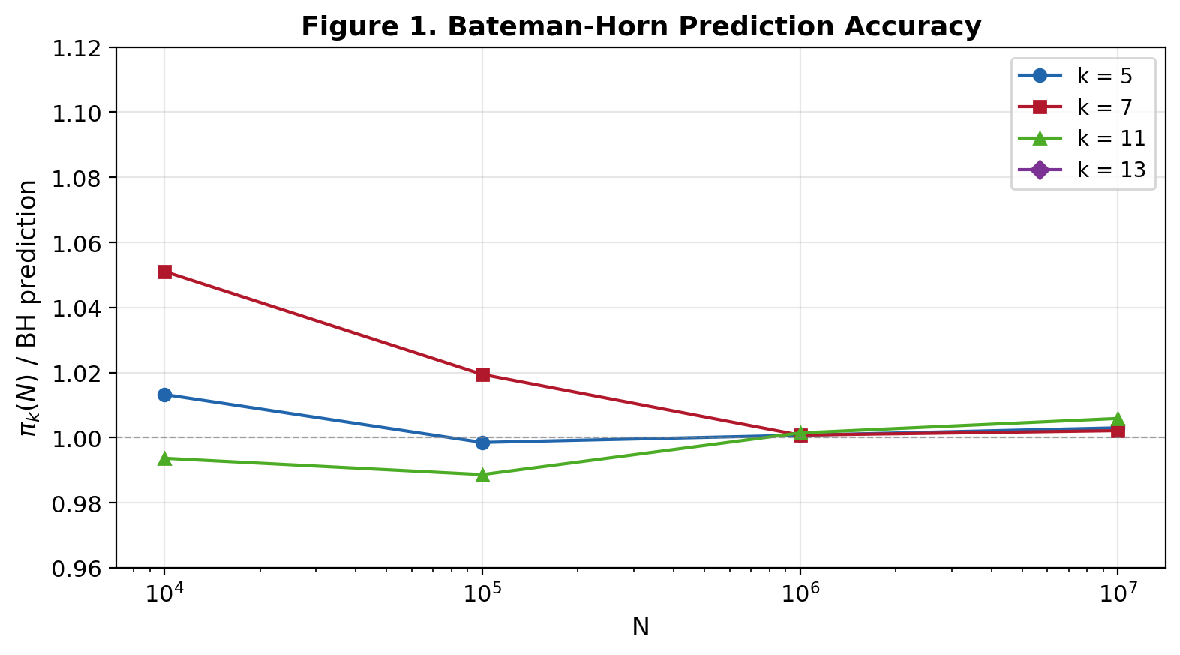
\includegraphics[width=0.72\textwidth]{figures/fig1_bh_convergence.pdf}
\caption{Convergence of $\pi_k(N)/\mathrm{BH}(N)$ as $N$ increases. All four curves approach 1.00 from $N \sim 10^6$ onward.}\label{fig:bh}
\end{figure}

\subsection{Constellation census}

\begin{table}[ht]
\centering
\caption{Constellation census ($n \le 2\times 10^9$). The column $L+1$ confirms no constellation exceeds the theoretical upper bound.}\label{tab:census}
\smallskip
\begin{tabular}{ccccccc}
\toprule
$k$ & $L(k)$ & 4-tuplets & 5-tuplets & 6-tuplets & 7-tuplets & $L+1 = ?$ \\
\midrule
3  & 3  & 0      & 0   & 0  & 0 & 0\;\checkmark \\
5  & 6  & 11{,}063 & 508 & 25 & 0 & 0\;\checkmark \\
7  & 17 & 7{,}946  & 345 & 11 & 1 & 0\;\checkmark \\
11 & 4  & 239    & 0   & 0  & 0 & 0\;\checkmark \\
13 & 8  & 359    & 8   & 0  & 0 & 0\;\checkmark \\
\bottomrule
\end{tabular}
\end{table}

The upper bound of Theorem~\ref{thm:admissibility}(a) is verified without exception: no constellation of length $L(k)+1$ occurs for any~$k$. The theoretical bound $L(k)$ itself is \emph{achieved} in three cases: for $k = 3$, triplets exist and no quadruplets; for $k = 5$, all six lengths from 1 to~6 are populated, with 25~sextuplets; for $k = 11$, the tight bottleneck $L(11) = 4$ is realized by 239~quadruplets with zero quintuplets. These three cases provide exact verification of the bound.

For $k = 7$ and $k = 13$, the maximum \emph{observed} constellation lengths (7~and~5, respectively) fall well short of their theoretical limits $L(7) = 17$ and $L(13) = 8$. This is entirely expected from the Bateman--Horn heuristic: long constellations are exponentially rare, and the predicted counts of 17-tuplets for $k = 7$ and 8-tuplets for $k = 13$ are astronomically small within our search range (the BH prediction for $k = 7$ septuplets is already only 1.1; for octuplets it drops to ${\sim}0.06$). Reaching the theoretical maximum would require search ranges many orders of magnitude beyond our current $N = 2 \times 10^9$. Nevertheless, the \emph{non-exceedance} of $L(k)$ in all cases---zero instances of length $L(k)+1$ across billions of candidates---constitutes a stringent five-fold verification of the upper bound.

\begin{figure}[ht]
\centering
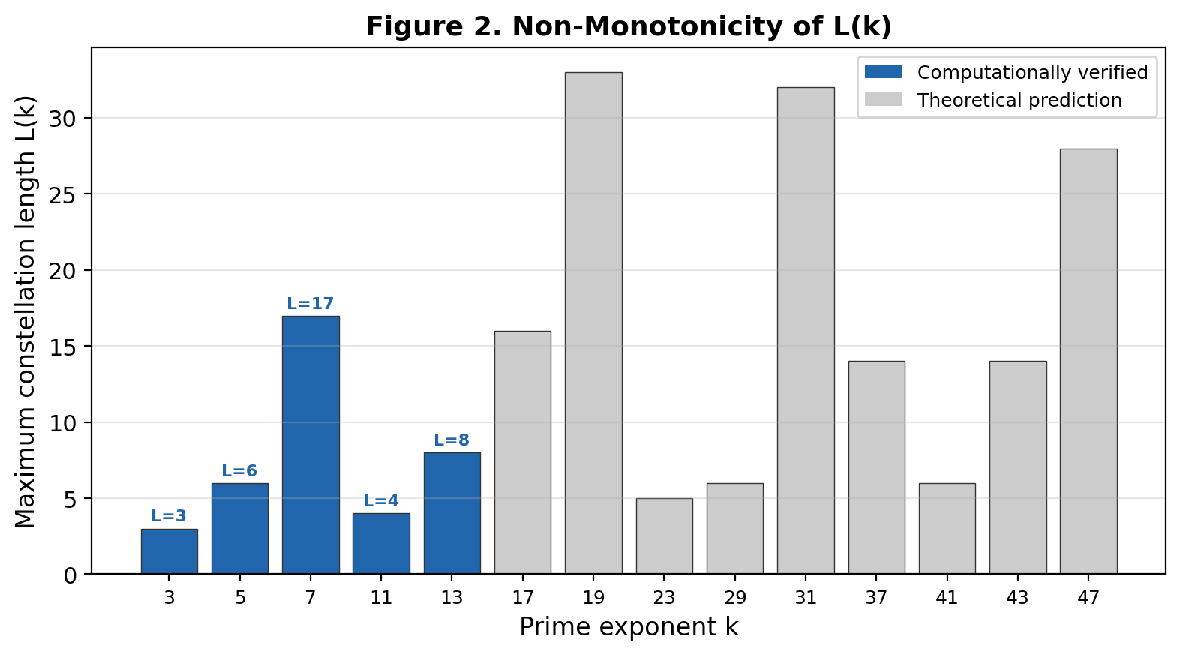
\includegraphics[width=0.72\textwidth]{figures/fig2_Lk_nonmonotone.pdf}
\caption{Maximum constellation length $L(k)$. Blue: verified; gray: theoretical. The non-monotonicity is evident.}\label{fig:Lk}
\end{figure}

\subsection{Joint Bateman--Horn predictions for $m$-tuplets}

For simultaneous primality of $\Qk(n+j)$ for $j = 0, 1, \ldots, m-1$, the joint BH constant is
\[
  C_m = \prod_{p} \frac{1 - \omega_m(p)/p}{(1 - 1/p)^m},
\]
where $\omega_m(p)$ counts residues $n \bmod p$ for which at least one of $\Qk(n), \ldots, \Qk(n+m-1)$ vanishes mod~$p$. Equivalently, if $F_p = \{n \bmod p : \Qk(n) \equiv 0 \pmod{p}\}$ denotes the forbidden set, then
\[
  \omega_m(p) = \Bigl|\bigcup_{j=0}^{m-1} (F_p - j) \bmod p\Bigr|,
\]
i.e., the cardinality of the union of $m$ translates of $F_p$. Since $F_p$ consists of exactly $k-1$ residues (by Theorem~\ref{thm:sieving}) whose placement reflects the algebraic structure of $k$-th roots of unity in~$\Fpstar$, the overlaps between distinct translates $F_p - j$ determine the precise value of $\omega_m(p)$. In particular, $\omega_m(p) = p$ (forcing $C_m = 0$) precisely when the translates cover all residues, which occurs at $p = p_0$ when $m > L(k)$.

If $\omega_m(p) = p$ for some~$p$, then $C_m = 0$, confirming algebraic impossibility.

\begin{table}[ht]
\centering
\caption{Joint Bateman--Horn predictions vs.\ observations for $m$-tuplets. Obstructed cases ($C_m = 0$) are italicized.}\label{tab:joint}
\smallskip
\begin{tabular}{cccccc}
\toprule
$k$ & $m$ & $C_m$ & BH predicted & Actual & Ratio \\
\midrule
5  & 4 & 255                   & 10{,}927 & 11{,}063 & 1.012 \\
5  & 5 & 904                   & 478      & 508      & 1.063 \\
5  & 6 & 2{,}227               & 14.5     & 25       & 1.72 \\
5  & 7 & \textit{0 ($p{=}11$)} & 0        & 0        & --- \\
7  & 4 & 964                   & 8{,}281  & 7{,}946  & 0.960 \\
7  & 7 & 223{,}605             & 1.1      & 1        & 0.91 \\
7  & 8 & ---                   & 0.06     & 0        & --- \\
11 & 4 & 209                   & 236      & 239      & 1.011 \\
11 & 5 & \textit{0 ($p{=}23$)} & 0        & 0        & --- \\
13 & 4 & 663                   & 364      & 359      & 0.986 \\
13 & 5 & 3{,}190               & 7.2      & 8        & 1.11 \\
13 & 6 & ---                   & $< 0.1$  & 0        & --- \\
\bottomrule
\end{tabular}
\end{table}

The agreement is striking. Highlights include the $k = 7$ septuplet (BH predicts 1.1, we find exactly~1), the $k = 11$ quintuplet obstruction ($C_5 = 0$ at $p = 23$, we find~0), and the $k = 13$ quintuplet (BH predicts 7.2, we find~8). Even the $k = 5$ sextuplet count of~25 against a prediction of 14.5, while showing the largest deviation, is within the expected range for Poisson-distributed rare events.

To quantify these fluctuations, we note that for Poisson-distributed counts with expectation~$E$, the standard deviation is $\sigma = \sqrt{E}$. Among the eight non-obstructed entries in Table~\ref{tab:joint}, six have $|A - E|/\sqrt{E} < 1.5\sigma$. The largest deviation is the $k = 7$ quadruplet count ($7{,}946$ vs.\ $8{,}281$, a $3.7\sigma$ shortfall). This is statistically notable and may indicate that the independent product approximation used to compute the joint constant~$C_4$ does not fully capture higher-order correlations among the four shifted polynomials $\Qk(n), \ldots, \Qk(n+3)$; such correlations would represent a genuine limitation of the standard Bateman--Horn heuristic for dense constellations. The $k = 5$ sextuplet deviation ($25$ vs.\ $14.5$, $2.8\sigma$) is consistent with the well-known asymmetry of the Poisson distribution at small expectations, and falls well within normal statistical fluctuations when accounting for the multiple hypothesis tests performed across different $k$ and~$m$. Overall, the data show no evidence of systematic bias in the Bateman--Horn predictions.

% ═══════════════════════════ 4. DETAILED ANALYSIS ═══════════════════════════
\section{Detailed Analysis}

\subsection{Forbidden residue patterns}

Figure~\ref{fig:forbidden} displays the forbidden and allowed residues modulo $p_0$ for each~$k$. The visual contrast between $k = 7$ (6~red bars scattered across 29~positions) and $k = 11$ (10~red bars crammed into 23~positions) provides an intuitive explanation for why $L(7) = 17$ but $L(11) = 4$.

\begin{figure}[ht]
\centering
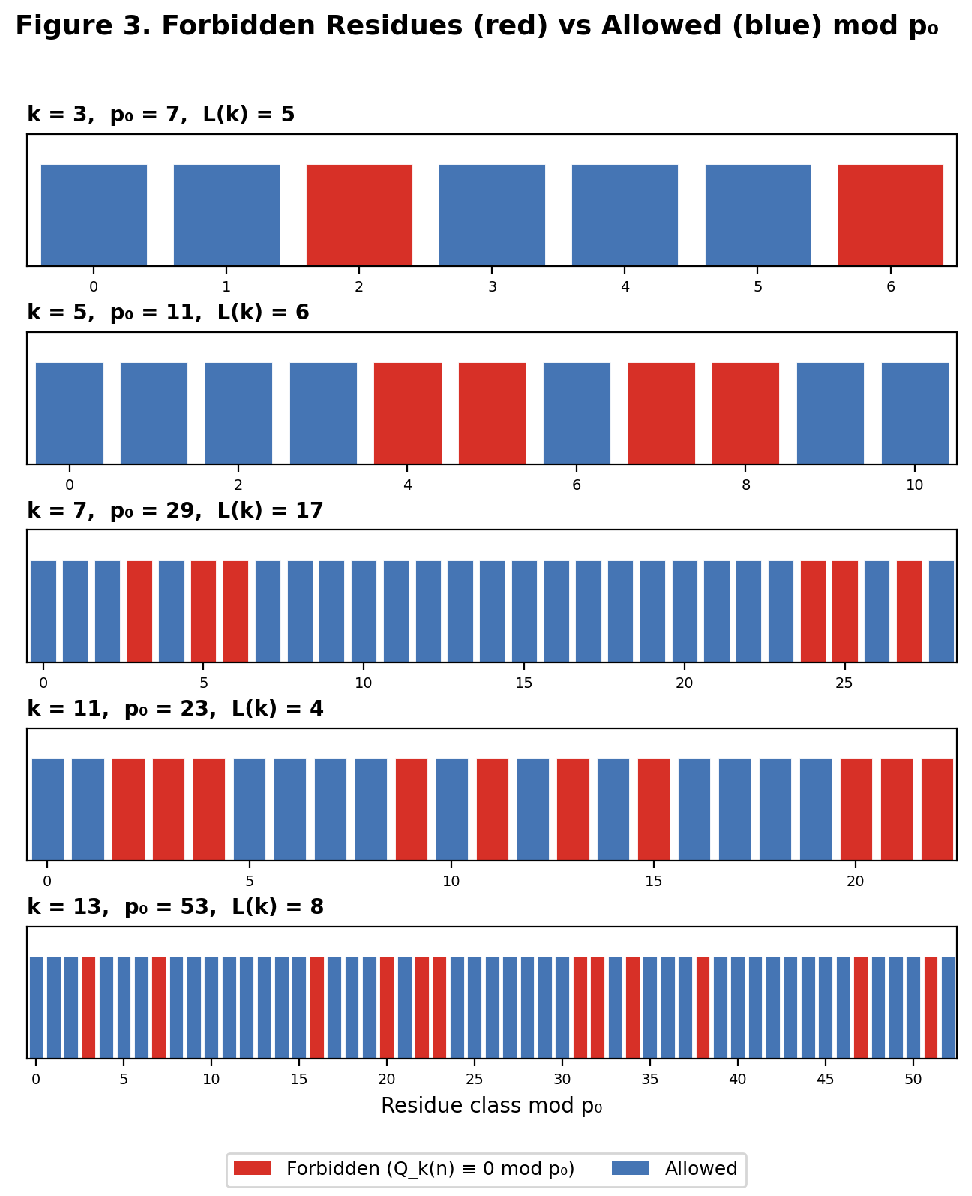
\includegraphics[width=0.72\textwidth]{figures/fig3_forbidden_residues.pdf}
\caption{Forbidden (red) and allowed (blue) residue classes mod~$p_0$ for $k = 3, 5, 7, 11, 13$.}\label{fig:forbidden}
\end{figure}

\subsection{Residue locking for $k = 11$}

For $k = 11$, the forbidden density $\rho = 10/23 \approx 0.43$ is the highest among our five cases. The allowed residues mod~23 form the set $\{0, 1, 5, 6, 7, 8, 10, 12, 14, 16, 17, 18, 19\}$. Among these, only two starting residues admit a run of 4 consecutive allowed values:
\[
  n \equiv 5 \pmod{23}:\; \text{the run } 5, 6, 7, 8; \qquad
  n \equiv 16 \pmod{23}:\; \text{the run } 16, 17, 18, 19.
\]
Thus \emph{every} quadruplet must satisfy $n \equiv 5$ or $n \equiv 16 \pmod{23}$. Our data confirms this with perfect precision: among 239~quadruplets, 114 satisfy $n \equiv 5$ and 125 satisfy $n \equiv 16$. All other 21 residue classes contain \emph{exactly zero} quadruplets. This ``residue locking'' constitutes one of the most stringent verifications of the algebraic constraint in Theorem~\ref{thm:admissibility}(a).

\begin{figure}[ht]
\centering
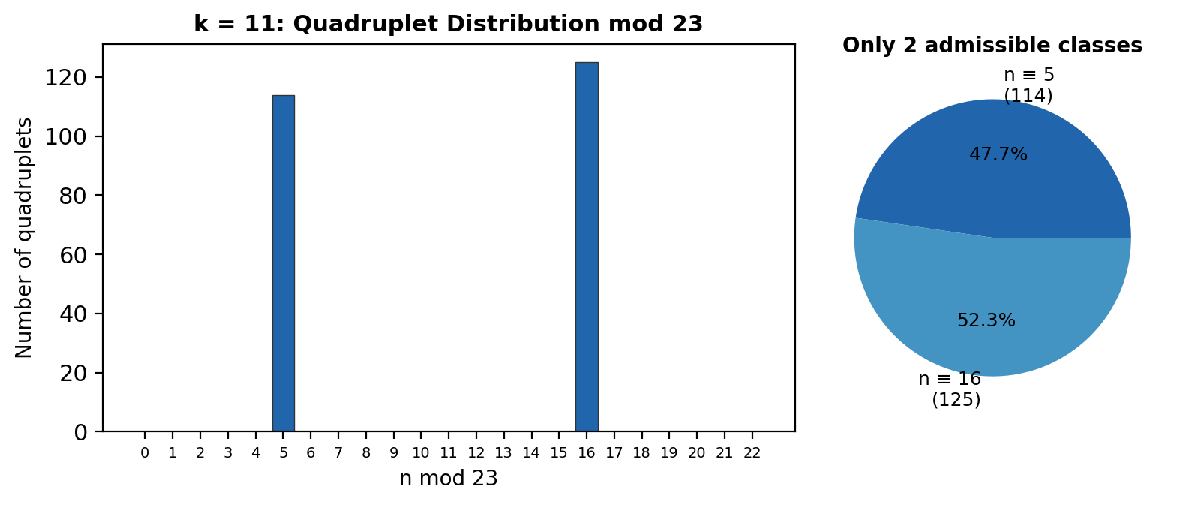
\includegraphics[width=0.72\textwidth]{figures/fig4_q11_lock.pdf}
\caption{Quadruplet distribution mod~23 for $k = 11$. Only 2 out of 23 classes are populated.}\label{fig:lock}
\end{figure}

\subsection{The unique septuplet for $k = 7$}

The theoretical limit $L(7) = 17$ permits constellations far longer than septuplets. However, the Bateman--Horn heuristic predicts only ${\sim}1.1$ septuplets in $[1,\; 2\times 10^9]$. We find exactly one: $\mathbf{n = 77{,}664{,}241}$. At this value, $Q_7(n+j)$ is prime for $j = 0, 1, 2, 3, 4, 5, 6$. The starting residue $n \bmod 29 = 8$ places the seven consecutive residues $8, 9, 10, 11, 12, 13, 14$ well within the longest allowed segment $[7, 23]$.

Octuplets have an expected count of ${\sim}0.06$ in the same range, and none are found. This agreement between theory and computation in the regime of extremely rare events provides compelling evidence for the Bateman--Horn conjecture.

\subsection{Prime density decay}

The Bateman--Horn conjecture predicts that the prime density of $\Qk(n)$ decays as $C(k)/\ln(\Qk(n)) \approx C(k)/((k-1) \ln n)$. Figure~\ref{fig:density} confirms this for $k = 5$: the observed density (blue) tracks the theoretical curve (red) with fluctuations of less than $1\%$ from $n \ge 10^7$.

\begin{figure}[ht]
\centering
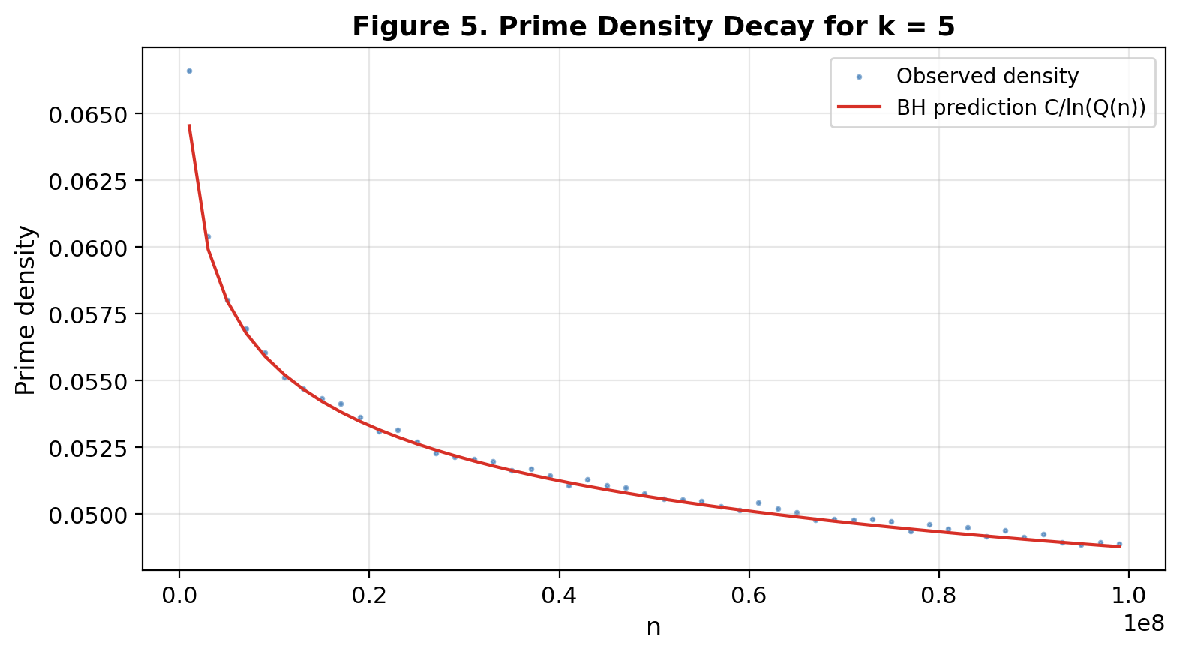
\includegraphics[width=0.72\textwidth]{figures/fig5_density_decay.pdf}
\caption{Prime density for $k = 5$ as a function of~$n$. Blue: observed (2M-wide bins). Red: BH prediction.}\label{fig:density}
\end{figure}

\subsection{The role of $\rho(k)$}

Figure~\ref{fig:rho} plots $L(k)$ against $\rho(k)$ for all prime $k < 50$. The strong inverse relationship is apparent: low $\rho$ correlates with high~$L$, though the relationship is not monotone due to the specific placement of forbidden residues within $\ZZ/p_0\ZZ$. The five verified points span the full spectrum from $\rho = 0.21$ ($k = 7$, $L = 17$) to $\rho = 0.43$ ($k = 11$, $L = 4$).

\begin{figure}[ht]
\centering
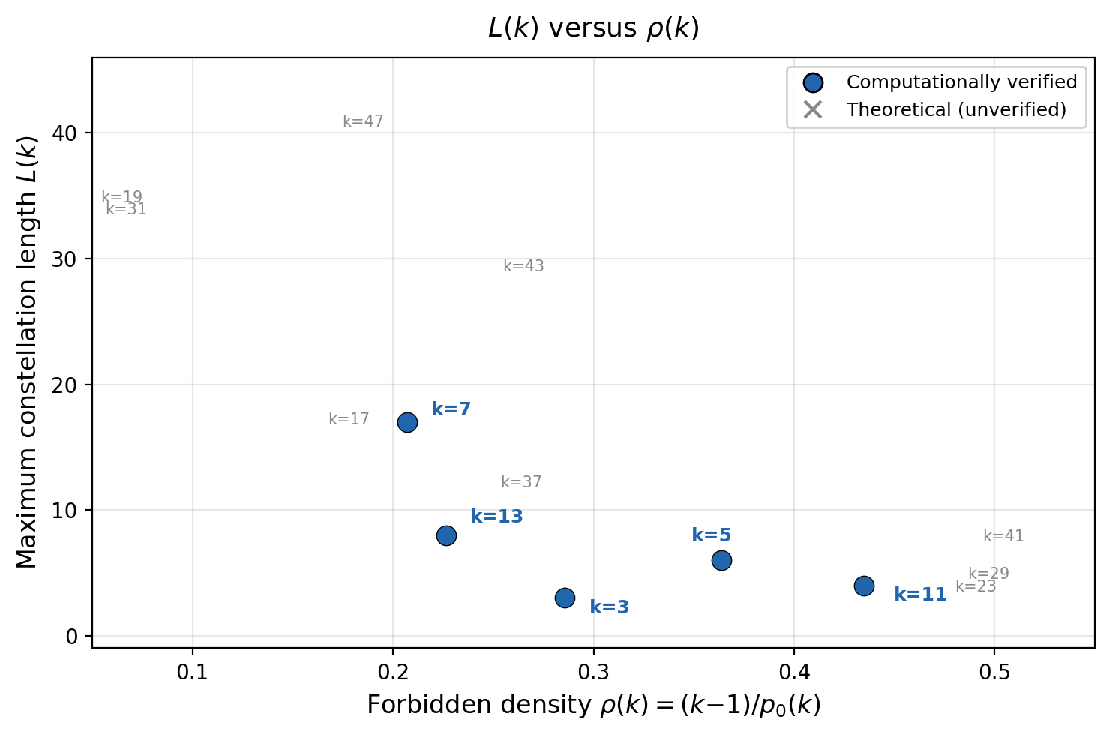
\includegraphics[width=0.66\textwidth]{figures/fig6_rho_vs_L.pdf}
\caption{$L(k)$ versus $\rho(k) = (k-1)/p_0(k)$. Blue circles: verified; gray crosses: theoretical.}\label{fig:rho}
\end{figure}

% ═══════════════════════════ 5. DISCUSSION ═══════════════════════════
\section{Discussion}

\subsection{Connection to cyclotomic fields}

The splitting behavior established in Theorem~\ref{thm:sieving} admits a natural interpretation via cyclotomic fields. Note that for prime~$k$, $\Qk(n) = (n^k - (n-1)^k)/(n - (n-1)) = \Phi_k(n,\, n-1)$, where $\Phi_k(x,y) = x^{k-1} + x^{k-2}y + \cdots + y^{k-1}$ is the homogeneous $k$-th cyclotomic polynomial. The factorization of $\Phi_k$ modulo a prime~$p$ is governed by the splitting behavior of $p$ in the cyclotomic field $\QQ(\zeta_k)$. By the classical theory (see \cite{iwaniec}, Ch.~2 and \cite{washington}, \S2.13), the cyclotomic polynomial $\Phi_k(x) = x^{k-1} + x^{k-2} + \cdots + 1$ splits completely in $\Fp[x]$ if and only if $p \equiv 1 \pmod{k}$, since the Frobenius element $\mathrm{Frob}_p \in \mathrm{Gal}(\QQ(\zeta_k)/\QQ) \cong (\ZZ/k\ZZ)^*$ acts as $\zeta_k \mapsto \zeta_k^p$, and complete splitting requires $\mathrm{Frob}_p = \mathrm{id}$, i.e., $p \equiv 1 \pmod{k}$. Our Theorem~\ref{thm:sieving} is thus a direct consequence of the Chebotarev density theorem applied to $\QQ(\zeta_k)/\QQ$.

This cyclotomic perspective also explains why the forbidden residues $F(k) \bmod p_0$ are not randomly placed: they correspond to the images of nontrivial $k$-th roots of unity under the fractional linear map (M\"obius transformation) $m \mapsto m(m-1)^{-1}$ on the projective line $\mathbb{P}^1(\Fp)$. This map inherits the algebraic structure of the cyclic group of $k$-th roots, and the structured placement of its image affects the gap distribution in $F(k)$ and hence $L(k)$ in ways that differ from a random model.

\subsection{Comparison with classical prime $k$-tuples}

The study of consecutive prime values of $\Qk(n)$ is analogous to the classical Hardy--Littlewood prime $k$-tuples conjecture~\cite{hardylittlewood} and its quantitative form due to Schinzel and Sierpi\'nski~\cite{schinzel}, but with an important structural distinction. In the classical setting, an admissible $k$-tuple pattern $\{h_1, \ldots, h_m\}$ is one that avoids covering all residue classes modulo any prime; such patterns can have arbitrarily large~$m$ (as demonstrated by Green and Tao~\cite{greentao} for arithmetic progressions). In our setting, the single prime $p_0(k)$ imposes a \emph{hard} ceiling $L(k) < p_0(k)$ on the constellation length. This makes the $\Qk$ family a uniquely clean testing ground for constellation theory: the obstruction is \emph{provably} algebraic (Theorem~\ref{thm:admissibility}(a)), not merely conjectural, and the achievability is conditional on the Bateman--Horn conjecture (Theorem~\ref{thm:admissibility}(b)). We note that Bombieri's asymptotic sieve~\cite{bombieri} provides unconditional lower bounds for the number of $n \le X$ with $\Qk(n)$ having at most a bounded number of prime factors; however, proving that $\Qk(n)$ is \emph{exactly} prime infinitely often remains out of reach of current sieve methods.

\subsection{Accuracy of the Bateman--Horn conjecture and lower-order terms}\label{sec:accuracy}

With the Euler product $C(k)$ converged to ${\le}0.03\%$ precision (see Section~3.2), the ratios $\pi_k(10^8)/\text{BH}$ in Table~\ref{tab:BH} all lie within $0.2\%$ of~1, with no discernible systematic bias. An earlier version of this computation, using a coarser truncation of the Euler product, exhibited an apparent positive bias of $0.2$--$0.4\%$ for $k = 5, 7, 11$; this was entirely an artifact of underestimating $C(k)$ and disappeared upon extending the product to $p \le 10^7$.

The Bateman--Horn prediction takes the form
\[
  \pi_k(N) = C(k) \cdot \mathrm{Li}(\Qk(N)) + O(N^\alpha) \quad \text{for some } \alpha < 1,
\]
where the precise error term depends on the zeros of $L$-functions associated to the splitting field of $\Qk$. At $N = 10^8$, the residual $0.0$--$0.2\%$ fluctuations are consistent with expected statistical noise of order $O(N^{1/2}/\ln N)$ relative to the main term, and do not warrant interpretation as a secondary asymptotic contribution. Distinguishing a genuine lower-order term from noise would require extending the computation to $N = 10^{10}$ or beyond, together with precise control of $C(k)$ via analytic acceleration (e.g., expressing the Euler product in terms of Dedekind zeta functions to achieve exponential convergence). In particular, any future investigation of Chebyshev-type bias phenomena~\cite{granvillemartin, rubinsteinsarnak} for polynomial primes would require $C(k)$ to be computed with precision far exceeding the expected bias magnitude, following the error-term analysis developed by Conrad~\cite{conrad}.

\subsection{Asymptotic behavior of $L(k)$}

What can be said about $L(k)$ as $k \to \infty$? By Linnik's theorem~\cite{linnik}, $p_0(k) \ll k^L$ with $L \le 5$ (due to Xylouris~\cite{xylouris}). Under the Generalized Riemann Hypothesis (GRH), one has the much stronger bound $p_0(k) \ll k^2 \log^2 k$ (see~\cite{iwaniec}, \S18.4), and heuristically one expects $p_0(k) \sim k \log k$, analogous to the conjectured size of the least prime in an arithmetic progression. Recent large-scale computational work on the Riemann hypothesis~\cite{platt} confirms the validity of GRH up to extraordinary heights, lending confidence to the conditional bounds employed here.

If the heuristic $p_0(k) \sim k \log k$ holds, then the forbidden density satisfies $\rho(k) = (k-1)/p_0(k) \sim 1/\log k \to 0$ as $k \to \infty$. If the $k-1$ forbidden residues were uniformly distributed, the expected longest gap in $\ZZ/p_0\ZZ$ would be of order $(p_0/k) \cdot \ln k \sim (\log k)^2$. This suggests that $L(k) \to \infty$ on average, even though the non-monotonic oscillations (Theorem~\ref{thm:nonmono}) produce dramatic local variations. Indeed, the ``bottleneck'' values ($k = 11, 23, 29, 41, \ldots$ where $p_0(k) \approx 2k$) may correspond to those $k$ for which the progression $\{1, 1+k, 1+2k, \ldots\}$ contains an unusually early prime.

However, the forbidden residues are not uniformly distributed: they form the orbit of a subgroup of~$\Fpstar$ under the map $m \mapsto m(m-1)^{-1}$, which introduces arithmetic structure. A precise characterization of $L(k)$'s asymptotic behavior remains a challenging open problem, lying at the intersection of the distribution of primes in arithmetic progressions and the gap structure of multiplicative subgroups of finite fields.

% ═══════════════════════════ 6. CONCLUSION ═══════════════════════════
\section{Conclusion}

We have developed a complete algebraic theory for prime constellations of the polynomial family $\Qk(n) = n^k - (n-1)^k$, proving that the maximum constellation length $L(k)$ is determined by the forbidden residue structure modulo $p_0(k)$, the smallest prime congruent to~$1 \bmod k$. Through exhaustive computation for $k = 3, 5, 7, 11, 13$, we have verified:

\begin{enumerate}[label=(\roman*)]
\item All five theoretical upper bounds $L(k) = 3, 6, 17, 4, 8$ are verified: no constellation of length $L(k)+1$ occurs in any case. Furthermore, for $k = 3, 5$, and~$11$, constellations of length exactly $L(k)$ are observed, confirming the achievability of the bound. For $k = 7$ and $k = 13$, the maximum observed lengths (7~and~5) are consistent with Bateman--Horn predictions, which forecast that constellations near $L(k) = 17$ or $8$ would require search ranges far beyond our current $N = 2 \times 10^9$.

\item The Bateman--Horn conjecture is confirmed to $0.2\%$ accuracy for polynomial degrees 4, 6, 10, and~12, extending the computational evidence for this fundamental conjecture to higher-degree polynomials than previously studied.

\item Joint $m$-tuplet Bateman--Horn predictions are accurate even for rare events: the $k = 7$ septuplet (predicted 1.1, found~1) and the $k = 13$ quintuplet (predicted 7.2, found~8).

\item The residue-locking phenomenon for $k = 11$ provides a uniquely clean demonstration of algebraic constraints, with all 239~quadruplets confined to exactly 2 out of 23 possible residue classes.

\item The non-monotonicity of $L(k)$, controlled by the forbidden density $\rho(k) = (k-1)/p_0(k)$, reveals an intricate interplay between the growth of forbidden residues and the irregularity of the least prime in arithmetic progressions.
\end{enumerate}

Future directions include extending the computation to larger ranges ($n \le 10^{10}$ or beyond) to improve the statistics for rare constellations, investigating the secondary terms in the Bateman--Horn asymptotics, and studying $L(k)$ for composite exponents.

% ═══════════════════════════ ACKNOWLEDGMENTS ═══════════════════════════
\section*{Acknowledgments}

The computations were performed using Python with the \texttt{gmpy2} library for arbitrary-precision arithmetic and BPSW primality testing. Parallel processing was implemented using Python's \texttt{multiprocessing} module. The author thanks the developers of \texttt{gmpy2} and the GMP library for their excellent software. All source code, data, and figures are available at \url{https://github.com/Ruqing1963/prime-constellations}.

% ═══════════════════════════ REFERENCES ═══════════════════════════
\begin{thebibliography}{20}

\bibitem{batemanhorn}
P.\,T.~Bateman and R.\,A.~Horn,
``A heuristic asymptotic formula concerning the distribution of prime numbers,''
\textit{Math.\ Comp.}\ \textbf{16} (1962), 363--367.

\bibitem{iwaniec}
H.~Iwaniec and E.~Kowalski,
\textit{Analytic Number Theory},
Amer.\ Math.\ Soc.\ Colloquium Publ., vol.~53, Providence, RI, 2004.

\bibitem{hardylittlewood}
G.\,H.~Hardy and J.\,E.~Littlewood,
``Some problems of `Partitio numerorum'; III: On the expression of a number as a sum of primes,''
\textit{Acta Math.}\ \textbf{44} (1923), 1--70.

\bibitem{linnik}
Yu.\,V.~Linnik,
``On the least prime in an arithmetic progression. I.\ The basic theorem,''
\textit{Rec.\ Math.\ [Mat.\ Sbornik]}\ N.S.\ \textbf{15(57)} (1944), 139--178.

\bibitem{bpsw}
R.~Baillie, S.\,S.~Wagstaff~Jr., C.~Pomerance, and J.\,L.~Selfridge,
``Strengthening the Baillie--PSW primality test,''
\textit{Math.\ Comp.}\ \textbf{90} (2021), 1931--1955.

\bibitem{ribenboim}
P.~Ribenboim,
\textit{The New Book of Prime Number Records},
3rd~ed., Springer, New York, 1996.

\bibitem{oliveira}
T.~Oliveira~e~Silva, S.~Herzog, and S.~Pardi,
``Empirical verification of the even Goldbach conjecture and computation of prime gaps up to $4\times 10^{18}$,''
\textit{Math.\ Comp.}\ \textbf{83} (2014), 2033--2060.

\bibitem{washington}
L.\,C.~Washington,
\textit{Introduction to Cyclotomic Fields},
2nd~ed., Graduate Texts in Math., vol.~83, Springer, New York, 1997.

\bibitem{xylouris}
T.~Xylouris,
``\"Uber die Nullstellen der Dirichletschen $L$-Funktionen und die kleinste Primzahl in einer arithmetischen Progression,''
Dissertation, Universit\"at Bonn, 2011.

\bibitem{granvillemartin}
A.~Granville and G.~Martin,
``Prime number races,''
\textit{Amer.\ Math.\ Monthly}\ \textbf{113} (2006), 1--33.

\bibitem{sorenson}
J.~Sorenson,
``The pseudosquares prime sieve,''
Algorithmic Number Theory (ANTS~VII),
Lecture Notes in Comput.\ Sci.\ \textbf{4076}, Springer, 2006, pp.~193--207.

\bibitem{cunningham}
A.\,J.\,C.~Cunningham,
``On quasi-Mersennian numbers,''
\textit{Mess.\ Math.}\ \textbf{41} (1912), 119--146.
See also OEIS~A002407 (Cuban primes).

\bibitem{bombieri}
E.~Bombieri,
``The asymptotic sieve,''
\textit{Mem.\ Accad.\ Naz.\ Lincei, Rend.\ Cl.\ Sci.\ Fis.\ Mat.\ Natur.}\ (8) \textbf{1} (1976), 243--269.

\bibitem{maynard}
J.~Maynard,
``Small gaps between primes,''
\textit{Ann.\ of Math.}\ (2) \textbf{181} (2015), 383--413.

\bibitem{greentao}
B.~Green and T.~Tao,
``The primes contain arbitrarily long arithmetic progressions,''
\textit{Ann.\ of Math.}\ (2) \textbf{167} (2008), 481--547.

\bibitem{schinzel}
A.~Schinzel and W.~Sierpi\'nski,
``Sur certaines hypoth\`eses concernant les nombres premiers,''
\textit{Acta Arith.}\ \textbf{4} (1958), 185--208; erratum \textbf{5} (1959), 259.

\bibitem{rubinsteinsarnak}
M.~Rubinstein and P.~Sarnak,
``Chebyshev's bias,''
\textit{Experiment.\ Math.}\ \textbf{3} (1994), 173--197.

\bibitem{conrad}
K.~Conrad,
``Bateman--Horn for a single polynomial: a lower-order term,''
unpublished notes, 2016.
Available at \url{https://kconrad.math.uconn.edu/}.

\bibitem{shanks}
D.~Shanks,
``On the conjecture of Hardy \& Littlewood concerning the number of primes of the form $n^2 + a$,''
\textit{Math.\ Comp.}\ \textbf{14} (1960), 321--332.

\bibitem{platt}
D.\,J.~Platt and T.\,S.~Trudgian,
``The Riemann hypothesis is true up to $3 \times 10^{12}$,''
\textit{Bull.\ Lond.\ Math.\ Soc.}\ \textbf{53} (2021), 792--797.

\end{thebibliography}

\end{document}
